%% ceci est un commentaire 
%% il faut toujours commencer par \documentclass[type de papier, taille de texte]{sytle du document}
\documentclass[a4paper,10pt]{report} %%%% sytle du document : report/book/article


%%%%%%%%%%%%%%%%%%%%%%%%%%%%%%%%%%%%%%%%%%%%%%%%%%%%%%%%%%%%%%%%%%%%%%%%%%%%%%%
%% la suite est une collection des "package" ou des "librararies" pour utiliser des codes spécifiques

%% il vous suffit de les copie-coller quand vous créez un nouveau document TeX (ou bien en ajouter plus si besoin).
\usepackage[utf8]{inputenc} %% pour les accents en français
\usepackage[frenchb]{babel} %% pour un format français
\usepackage{graphicx} %% pour afficher des graphiques
\usepackage{amsmath} %% pour écrire des symboles (maths), des équations, etc.
\usepackage{amssymb}
\usepackage{color}
\usepackage{bm} %% pour lister des citations/la biblio
\usepackage{hyperref} %% pour inserer des liens internet
\usepackage{cleveref} %% pour faire des références uax équations, tableaux, etc.
%\usepackage{setspace} %% pour changer l'espace entre les lignes
%\linespread{1.6} %% pour changer l'espace entre les lignes












%%%%%%%%%%%%%%%%%%%%%%%%%%%%%%%%%%%%%%%%%%%%%%%%%%%%%%%%%%%%%%%%%%%%%%%%%%%%%%%
\title{--------\textbf{Ecoulement bloqué}--------} %% choissez un titre approprié à votre sujet
\author{par\\ZHANG Xunjie\\pour le Méthodes numériques pour les EDP M1 } %% utilisez \\ pour une novuelle ligne
\date{fait le 06 avril 2017} %% pour afficher la date actuelle commenter cette ligne














%%%%%%%%%%%%%%%%%%%%%%%%%%%%%%%%%%%%%%%%%%%%%%%%%%%%%%%%%%%%%%%%%%%%%%%%%%%%%%%
%% TOUT ce qui va dans votre rapport doit être entre \begin{document} & \end{document}
\begin{document}
\selectlanguage{french} %% format français
\maketitle %% pour afficher le titre
\tableofcontents %% pour afficher/compiler le sommaire automatiquement
\listoffigures %% pour lister les figures
%%%%%%%%%%%%%%%%%%%%%%%%%%%%%%%%%%%%%%%%%%%%%%






%%%%%%%%%%%%%%%%%%%%%%%%%%%%%%%%%%%%%%%%%%%%%%
\chapter{Problème physique} %% pour commencer un chapitre

\section{Petite Annonce}
Dans cette séance de TP EDP , on veur calculer l'écoulement parallelle instationnaire $u(x,y)$ dans la direction $x$ , entre deux plans stationnaires qui se trouvent à $y=0$ et $y=h$. Avant $t=0$, l'écoulement est forcé par un gradient de pression $\frac{\partial p}{\partial x}=-\rho G$, mais à $t \geq0$ le gradient de pression $\frac{\partial p}{\partial x}$ est zéro . Enfin , c'est un modèle d'un écoulement bloqué du coup à $t=0$ .\\

pour moi ,$G=8.40$ \\

\section{Rappel}
De façon générale, le bilan de la quantité de mouvement s'exprime sous la forme :
\begin{equation}
\frac{\partial(\rho\overrightarrow{v})}{\partial t}+\overrightarrow{\nabla}\cdot(\rho\overrightarrow{v}\bigotimes\overrightarrow{v})=-\overrightarrow{\nabla}p+\overrightarrow{\nabla}\cdot\tau+\rho\overrightarrow{v}
\end{equation}


 On fait evolution dans le $x$ direction , et on assume :
 \begin{equation}
 \frac{\partial u}{\partial t}+\mu\frac{\partial u}{\partial x}+\omega\frac{\partial u}{\partial z}=-\frac{1}{\rho}\frac{\partial P}{\partial x}+\nu\Big(\frac{\partial^2 u}{\partial x^2}+\frac{\partial^2 u}{\partial y^2}\Big)+g_x
 \end{equation}
 
 
 On simplifie cette équation :
\begin{itemize}
    \item[$\bullet$]instationnnaire écoulement ,$\frac{\partial u}{\partial t}\neq0$
    \item[$\bullet$]écouplement plaine , $u$ est independent que $x$
    \item[$\bullet$]écoulement idirectional  $v=0$ , $w=0$
    \item[$\bullet$]à $t \geq0$ le gradient de pression $\frac{\partial p}{\partial x}$ est zéro
    \item[$\bullet$]la force volumique suivant la direction x est null
\end{itemize}


On trouve l'équation ci-dessous :
\begin{equation}
\frac{\partial u}{\partial t}=\nu\frac{\partial^2u}{\partial y^2}
\end{equation}

\section{Conditions}
Dans l'annonce ci-dessus on peut trouver condition innitiale , à l'instant $t=0$ :
$$\frac{\partial p}{\partial x}=0$$
pour la condition limite :
$$u(0,t)=u(h,t)=0$$


%%%%%%%%%%%%%%%%%%%%%%%%%%%%%%%%%%%%%%%%%%%
\chapter{Solution analytique}
On rappel la problème :
\begin{equation}
	\left\{
    \begin{array}{r c l }
        &\frac{\partial u}{\partial t}=\nu\frac{\partial^2u}{\partial y^2}\\
        &u(0,t)=u(h,t)=0 \, ,t>0\\
        &u(y,0)=C(y)
    \end{array}
    \right.
\end{equation}


On utilise la méthode de séparation de variables pour trouver la solution ananlytique :

$$u(y,t)=f(t)g(y)$$

et on trouve :

$$\frac{f''(t)}{f(t)}=\beta\nu$$
$$\frac{g''(y)}{g(y)}=\beta$$

La solution élémenttaire peut être écrit sous la form :

$$u_n(y,t) =C_ne^{-\nu(\frac{n\pi}{h})^2t}\sin(\frac{n\pi}{h}x)$$

La solution générale s'écrivent :
\begin{equation}
u(y,t)=\sum\limits_{n=1}^{\infty}u_n(y,t)=\sum\limits_{n=1}^{\infty}C_ne^{-\nu(\frac{n\pi}{h})^2t}\sin(\frac{n\pi}{h}x)
\label{equ_gene}
\end{equation}

Comment touver $C_n$ ? 

On utilise une truc ci-dessus :

$$\int_0^\pi\sin(nx)\sin(mx)dx=0 \, , m=n $$

à $t=0$ , on fait integral à droite et à gauche en mçeme temps pour l'équation \ref{equ_gene} :

\begin{equation}
C_n=\frac{2}{h}\int_0^hC(y)\sin(\frac{n\pi}{h}y)dy
\end{equation}

On prend $C_n=\frac{4Gh^2}{k^3\pi^3\nu} $ pour la partie suivante .





%%%%%%%%%%%%%%%%%%%%%%%%%%%%%%%%%%%%%%%%%%%%%%
\chapter{Méthode numérique}
On utilise $\theta$ schéma pour la simulation numérique :

\begin{equation}
\frac{u_i^{n+1}-u_i^n}{\triangle t}=\theta\nu\frac{u_{i+1}^{n}-2u_i^n+u_{i-1}^n}{\triangle y^2}+(1-\theta)\nu\frac{u_{i+1}^{n+1}-2u_i^{n+1}+u_{i-1}^{n+1}}{\triangle y^2}
\end{equation}

Commentez :

\begin{itemize}
    \item[$\bullet$] $\theta=0$ , tous les terms evaluat à l'instant $t_{n+1}$ , implicite schéma .
    \item[$\bullet$]$\theta=1$ , tous les terms evaluat à l'instant $t-{n}$, explicite schéma .
    \item[$\bullet$]$\theta=\frac{1}{2} $ evaluat moyenne , Crank-Nicolson schémma .
\end{itemize}

Stabilité :

$$\frac{\psi^{n+1}}{\psi^n}=\frac{1-4\theta\nu\sin^2(\frac{\omega dx}{2})}{1+4(1-\theta)\nu\sin^2(\frac{\omega dx}{2})}$$

Dans l'annonce , $r=\frac{\nu\triangle t}{\triangle y^2}$ ,

$$0\leq r\leq\frac{1}{2}$$

%%%%%%%%%%%%%%%%%%%%%%%%%%%%%%%%%%%%%%%%%%%%%%
\chapter{Resultat}

\section{solution exact}
\begin{figure}[h]
%% [h] implique que le graphique sera placé ici (et pas en haut ou en bas du document)
\begin{center}
%% pour centré l'image
%	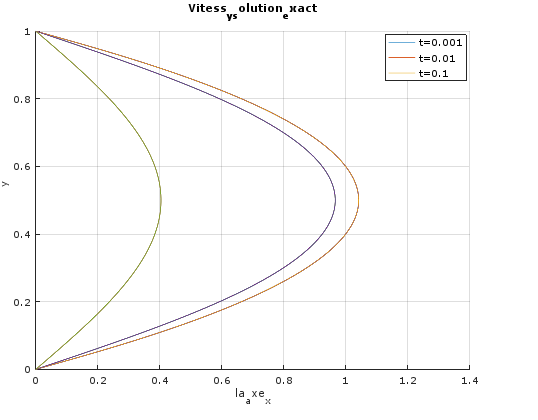
\includegraphics[width=1.0\textwidth]{FIG/figure3.png}
	%% 0.35 fois le largeur du document (\textwidth)
\end{center}
\caption{solution exact}
\label{fig:figureCoorPol}
\end{figure}

\section{solution nu-1 et nu-10}
\begin{figure}[h]
%% [h] implique que le graphique sera placé ici (et pas en haut ou en bas du document)
\begin{center}
%% pour centré l'image
%	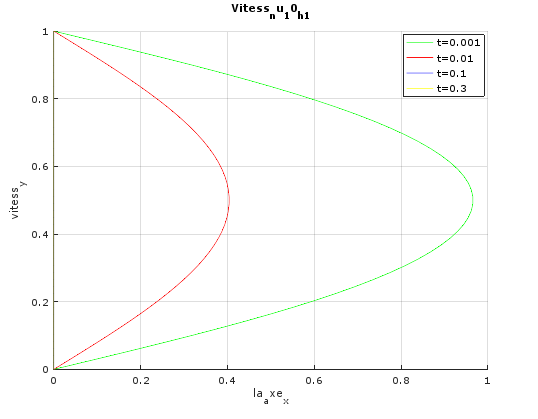
\includegraphics[width=1.0\textwidth]{FIG/figure1.png}
	%% 0.35 fois le largeur du document (\textwidth)
\end{center}
\caption{solution nu 1}
\label{fig:figureCoorPol}
\end{figure}
\begin{figure}[h]
%% [h] implique que le graphique sera placé ici (et pas en haut ou en bas du document)
\begin{center}
%% pour centré l'image
%	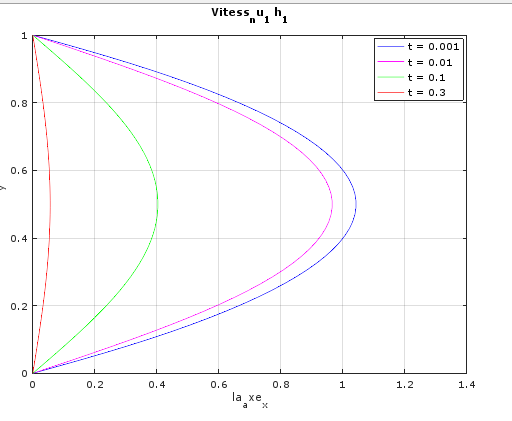
\includegraphics[width=1.0\textwidth]{FIG/figure2.png}
	%% 0.35 fois le largeur du document (\textwidth)
\end{center}
\caption{solution nu 10}
\label{fig:figureCoorPol}
\end{figure}


%%%%%%%%%%%%%%%%%%%%%%%%%%%%%%%%%%%%%%%%%%%%%%
%%%%%%%%%%%%%%%%%%%%%%%%%%%%%%%%%%%%%%%%%%%%%%
\chapter{Conclusion}

Dans cette séance de TP , on étude l'écoulement bloqué instationnaire . Au début on cherche la solution analytique de la problèm  , ensuite on fait une simulation utilisant $\theta$-schéma simulation numérique . On utilise Matlab pour programmer les solutions .

$\\$

Pour la précision , on dit que pour $\theta=\frac{1}{2}$ , la précision est $o(\triangle t^2, \triangle h^2)$ , par ailleur , la précision est $o(\triangle t, \triangle h)$ .







\bibliography{MonBiblio.bib}
\bibliographystyle{unsrtnat}	
\end{document}
\grid
